% -----------------------------------------------
% Template for SMC 2012
% adapted from the template for SMC 2011, which was adapted from that of SMC 2010
% -----------------------------------------------

\documentclass{article}
\usepackage{smc2015}
\usepackage{times}
\usepackage{ifpdf}
\usepackage[english]{babel}
\usepackage{cite}

\hyphenation{Java-script}

%%%%%%%%%%%%%%%%%%%%%%%% Some useful packages %%%%%%%%%%%%%%%%%%%%%%%%%%%%%%%
%%%%%%%%%%%%%%%%%%%%%%%% See related documentation %%%%%%%%%%%%%%%%%%%%%%%%%%
%\usepackage{amsmath} % popular packages from Am. Math. Soc. Please use the 
%\usepackage{amssymb} % related math environments (split, subequation, cases,
%\usepackage{amsfonts}% multline, etc.)
%\usepackage{bm}      % Bold Math package, defines the command \bf{}
%\usepackage{paralist}% extended list environments
%%subfig.sty is the modern replacement for subfigure.sty. However, subfig.sty 
%%requires and automatically loads caption.sty which overrides class handling 
%%of captions. To prevent this problem, preload caption.sty with caption=false 
%\usepackage[caption=false]{caption}
%\usepackage[font=footnotesize]{subfig}


%user defined variables
\def\papertitle{WEB AUDIO EVALUATION TOOL: A BROWSER-BASED LISTENING TEST ENVIRONMENT} %?
\def\firstauthor{Nicholas Jillings}
\def\secondauthor{Brecht De Man}
\def\thirdauthor{David Moffat}
\def\fourthauthor{Joshua D. Reiss}

% adds the automatic
% Saves a lot of ouptut space in PDF... after conversion with the distiller
% Delete if you cannot get PS fonts working on your system.

% pdf-tex settings: detect automatically if run by latex or pdflatex
\newif\ifpdf
\ifx\pdfoutput\relax
\else
   \ifcase\pdfoutput
      \pdffalse
   \else
      \pdftrue
\fi

\ifpdf % compiling with pdflatex
  \usepackage[pdftex,
    pdftitle={\papertitle},
    pdfauthor={\firstauthor, \secondauthor, \thirdauthor},
    bookmarksnumbered, % use section numbers with bookmarks
    pdfstartview=XYZ % start with zoom=100% instead of full screen; 
                     % especially useful if working with a big screen :-)
   ]{hyperref}
  %\pdfcompresslevel=9

  \usepackage[pdftex]{graphicx}
  % declare the path(s) where your graphic files are and their extensions so 
  %you won't have to specify these with every instance of \includegraphics
  \graphicspath{{./figures/}}
  \DeclareGraphicsExtensions{.pdf,.jpeg,.png}

  \usepackage[figure,table]{hypcap}

\else % compiling with latex
  \usepackage[dvips,
    bookmarksnumbered, % use section numbers with bookmarks
    pdfstartview=XYZ % start with zoom=100% instead of full screen
  ]{hyperref}  % hyperrefs are active in the pdf file after conversion

  \usepackage[dvips]{epsfig,graphicx}
  % declare the path(s) where your graphic files are and their extensions so 
  %you won't have to specify these with every instance of \includegraphics
  \graphicspath{{./figures/}}
  \DeclareGraphicsExtensions{.eps}

  \usepackage[figure,table]{hypcap}
\fi

%set up the hyperref package - make the links black without a surrounding frame
\hypersetup{
    colorlinks,%
    citecolor=black,%
    filecolor=black,%
    linkcolor=black,%
    urlcolor=black
}


% Title.
% ------
\title{\papertitle}

% Authors
% Please note that submissions are NOT anonymous, therefore 
% authors' names have to be VISIBLE in your manuscript. 
%
% Single address
% To use with only one author or several with the same address
% ---------------
%\oneauthor
%   {\firstauthor} {Affiliation1 \\ %
%     {\tt \href{mailto:author1@smcnetwork.org}{author1@smcnetwork.org}}}

%Two addresses
%--------------
% \twoauthors
%   {\firstauthor} {Affiliation1 \\ %
%     {\tt \href{mailto:author1@smcnetwork.org}{author1@smcnetwork.org}}}
%   {\secondauthor} {Affiliation2 \\ %
%     {\tt \href{mailto:author2@smcnetwork.org}{author2@smcnetwork.org}}}



% FIX!!! 
 \fourauthors
   {\firstauthor} {%Affiliation1 \\
     {\tt \href{mailto:b.deman@qmul.ac.uk}{n.g.r.jillings@se14.qmul.ac.uk, }}}
   {\secondauthor} {%Affiliation2\\ %
     {\tt \href{mailto:n.g.r.jillings@se14.qmul.ac.uk}{\{b.deman,}}}
   {\thirdauthor} {%Affiliation3\\ %
     {\tt \href{mailto:d.j.moffat@qmul.ac.uk}{d.j.moffat, }}}
    {\fourthauthor} {%Affiliation4\\ %
     {\tt \href{mailto:joshua.reiss@qmul.ac.uk}{joshua.reiss\}@qmul.ac.uk}}}

% ***************************************** the document starts here ***************
\begin{document}
%
\capstartfalse
\maketitle
\capstarttrue
%
\begin{abstract}
New functionality in HTML5, notably its Web Audio API, allows for increasingly powerful applications in the browser. % is this true?
Perceptual evaluation tests for audio, where the subject assesses certain qualities of different audio fragments through a graphical user interface and/or text boxes, require playback of audio and rapid switching between different files. % what else? 
The advantage of a web application is easy deployment on any platform, without requiring any other application or library, easy storing of results on a server. 
[...] % Need to expand here!
%Place your abstract at the top left column on the first page.
%Please write about 150-200 words that specifically highlight the purpose of your work,
%its context, and provide a brief synopsis of your results.
%Avoid equations in this part.\\

\end{abstract}

% TOTAL PAPER: Minimum 4 pages, 6 preferred, max. 8 (6 for demos/posters)\\ 

\section{Introduction}\label{sec:introduction}

%NICK: examples of what kind of audio applications HTML5 has made possible, with references to publications (or website)\\

Perceptual evaluation of audio plays an important role in a wide range of research including audio quality \cite{schoeffler2013impact,repp}, sound synthesis \cite{de2013real,durr2015implementation}, audio effect design \cite{deman2014a}, source separation \cite{uhlereiss}, music and emotion analysis \cite{song2013b,song2013a}, and many others \cite{friberg2011comparison}.  % codec design? 

The Web Audio API is a high-level JavaScript Application Programming Interface (API) designed for real-time processing of audio inside the browser through various processing nodes\footnote{http://webaudio.github.io/web-audio-api/}. Various web sites have used the Web Audio API for either creative purposes, such as drum machines and score creation tools\footnote{http://webaudio.github.io/demo-list/}, 
others from the list show real-time captured audio processing such as room reverberation tools and a phase vocoder from the system microphone. The BBC Radiophonic Workshop shows effects used on famous TV shows such as Doctor Who, being simulated inside the browser\footnote{http://webaudio.prototyping.bbc.co.uk/}. 
Another example is the BBC R\&D personalised compressor which applies a dynamic range compressor on a radio station that dynamically adjusts the compressor settings to match the listener's environment \cite{mason2015compression}. 

This work is based in part on the APE audio perceptual evaluation interface for MATLAB \cite{deman2014b}. An important drawback of this toolbox is the need to have MATLAB to create a test and even to run (barring the use of an executable generated by MATLAB), and limited compatibility with both earlier and newer versions of MATLAB, which makes it hard to maintain. On the other hand, a web application generally has the advantage of running in most browsers on most applications, and we present a tool that requires no specialised software or even programming knowledge to set up. 

% IMPORTANT
%[TO ADD: other interfaces for perceptual evaluation of audio, browser-based or not!] \\
%BROWSER-BASED: \cite{song2013b,song2013a,beaqlejs} \\
%MATLAB: \cite{whisper,mushram,scale}  
% to add: OPAQUE, Rumsey's repertory grid technique

Many perceptual audio interfaces are already available, such as the MATLAB-based tools MUSHRAM \cite{mushram}, WhisPER \cite{whisper}, and Scale \cite{scale}, and the browser-based tool used in \cite{song2013a,song2013b} and BeaqleJS \cite{beaqlejs}. The latter makes use of the HTML5 audio capabilities and comes with a number of predefined, established test interfaces such as ABX and MUSHRA \cite{mushra}. 
In this paper, we provide a listening test back end that allows for easy set up of a wide variety of listening tests, highly flexible yet very simple and not requiring any programming skills. 
% [How is this one different from all these?] improve

We present a browser-based perceptual evaluation tool from which any kind of multiple stimulus audio evaluation tool where subjects need to rank, rate, select, or comment on different audio samples can be built. 
We also include an example of the multiple stimulus user interface included with the APE tool \cite{deman2014b}, which presents the subject with a number of axes on which a number of markers, corresponding to audio samples, can be moved to reflect any subjective quality, as well as corresponding comment boxes. 
However, other graphical user interfaces can be put on top of the engine that we provide with minimal or no modifications. Examples of this are the MUSHRA test \cite{mushra}, single or multiple stimulus evaluation with a two-dimensional interface (such as valence and arousal dimensions), or simple annotation (using free-form text, check boxes, radio buttons or drop-down menus) of one or more audio samples at a time. 
In some cases, such as method of adjustment, where the audio is processed by the user \cite{bech}, or AB test \cite{bech}, where the interface does not show all audio samples to be evaluated at once, the back end of the tool needs to be modified as well. 

There are a number of advantages to building a web audio based listening test environment. The ability to easily deploy a flexible and scalable testing environment that requires no proprietary software to run makes the web audio evaluation tool a very flexible testing tool. The ability to host a single test server and create multiple clients not only allows multiple participants to be involved in a trial simultaneously, but also permits participants to be located anywhere in the world. There are also less user experience issues, since all users should have some experience with using existing web technologies.

In the following sections, we describe the included interface in more detail, discuss the implementation, and cover considerations that were made in the design process of this tool. 

\section{Interface}\label{sec:interface}

At this point, we have implemented the interface of the MATLAB-based APE (Audio Perceptual Evaluation) toolbox \cite{deman2014b}. This shows one marker for each simultaneously evaluated audio fragment on one or more horizontal axes, that can be moved to rate or rank the respective fragments in terms of any subjective quality, as well as a comment box for every marker, and any extra text boxes for extra comments. 
The reason for such an interface, where all stimuli are presented on a single rating axis (or multiple axes if multiple subjective qualities need to be evaluated), is that it urges the subject to consider the rating and/or ranking of the stimuli relative to one another, as opposed to comparing each individual stimulus to a given reference, as is the case with e.g. a MUSHRA test \cite{mushra}. See \ref{fig:interface} for an example of the interface, with eleven fragments and one axis. %? change if a new interface is shown

However, the back end of this test environment allows for many more established and novel interfaces for listening tests, particularly ones where the subject only assesses audio without manipulating it (i.e. method of adjustment), which would require additional features to be implemented. 

\begin{figure*}[ht]
\begin{center}
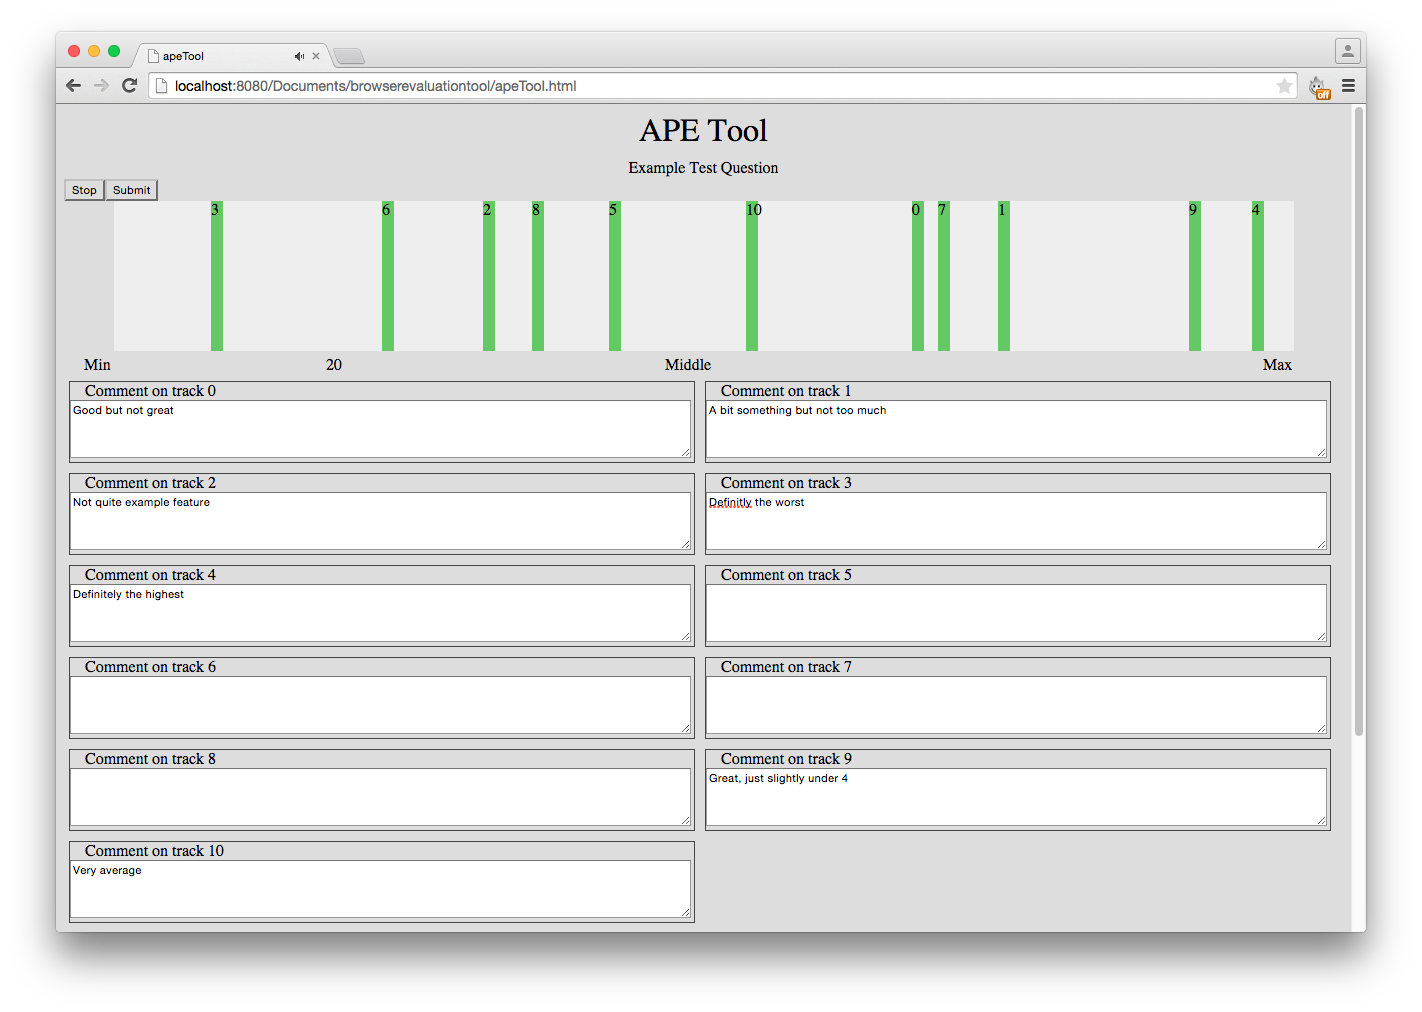
\includegraphics[width=0.9\textwidth]{interface.png}
\caption{Example of interface, with 1 axis and 11 fragments}
\label{fig:interface}
\end{center}
\end{figure*}


\section{Architecture}\label{sec:architecture} % or implementation? 

The tool runs entirely inside the browser through the new HTML5 Web Audio API and is supported by most major web browsers. The API allows for constructing audio processing elements and connecting them together to produce a high quality, real time signal process to manipulate audio streams. The API supports multichannel processing and has an accurate playback timer for precise scheduled playback control. The API is controlled through the browser JavaScript engine and is therefore highly configurable. Processing is all performed in a separate, low latency thread to the main JavaScript thread, so there is no blocking due to real time processing. 

The web tool itself is split into several files to operate:
\begin{itemize}
\item \texttt{index.html}: The main index file to load the scripts, this is the file the browser must request to load.
\item \texttt{core.js}: Contains functions and objects to define the audio objects, audio playback engine and loading media files
\item \texttt{ape.js}: Parses set up files to create the interface as instructed, following the same style chain as the MATLAB APE Tool \cite{deman2014b}.
\end{itemize}

The HTML file loads the \texttt{core.js} file along with a few other ancillary files (such as the jQuery JavaScript extensions\footnote{http://jquery.com/}), at which point the browser JavaScript begins to execute the on-page instructions, which gives the URL of the test set up XML document (outlined in Section \ref{sec:setupresultsformats}). \texttt{core.js} parses this document and executes the function in \texttt{ape.js} to build the web page with the given audio files. The reason for separating these two files is to allow for further interface designs (such as MUSHRA \cite{mushra} or AB tests \cite{bech}) to be used, which would still require the same underlying core functions outlined in \texttt{core.js}, see also Section \ref{sec:interface}.

The \texttt{ape.js} file has several main functions but the most important are \textit{loadInterface(xmlDoc)}, \textit{loadTest(id)}, \textit{pageXMLSave(testId)} and \textit{interfaceXMLSave()}. \textit{loadInterface(xmlDoc)} is called to decode the supplied project document in respect for the interface specified and define any global structures (such as the slider interface). It also identifies the number of pages in the test and randomises the order, if specified to do so. This is the only madatory function in any of the interface files as this is called by \texttt{core.js} when the document is ready. The design style is such that \texttt{core.js} cannot 'see' any interface specific functions and therefore cannot assume any are available. Therefore the \textit{loadInterface(xmlDoc)} is very important to set up the entire test environment. It can be assumed that the interface files can `see' the \texttt{core.js} file and can therefore not only interact with it, but also modify it.

Each test page is loaded using \textit{loadTest(id)} which performs two major tasks: to populate the interface with the slider elements and comment boxes; and secondly to instruct the \textit{audioEngine} to load the audio fragments and construct the backend audio graph. The markers on the slider at the top of the page are positioned randomly, to minimise the bias that may be introduced when the initial positions are near the beginning, end or middle of the slider. Another approach is to place the markers outside of the slider bar at first and have the subject drag them in, but the authors believe this doesn't encourage careful consideration and comparison of the different fragments as the implicit goal of the test becomes to audition and drag each fragment in just once, rather than to compare all fragments rigorously.

\textit{loadTest(id)} in \texttt{ape.js} also instructs the audio engine in \texttt{core.js} to create the \textit{audioObject} These are custom audio nodes, one representing each audio element specified in each page.
They consist of a \textit{bufferSourceNode} (a node which holds a buffer of audio samples for playback) and a \textit{gainNode}. There are various functions applied depending on metric collection which record the interaction with the audio element. These nodes are then connected to the \textit{audioEngine} (itself a custom web audio node) containing a \textit{gainNode} (where the various \textit{audioObject} connect to) for summation before passing the output to the \textit{destinationNode}, a permanent fixed node of the Web Audio API created as the master output where the browser then passes the audio information to the system sound device. % Does this now make sense?
% audio object/audioObject/Audio Object: -- should always be audioObject if talking about the JavaScript object, otherwise should say audio element or audio fragment.

When an \textit{audioObject} is created, it is given the URL of the audio sample to load. This is downloaded into the browser asynchronously using the \textit{XMLHttpRequest} object. This downloads any file into the JavaScript environment for further processing which is particularly useful for the Web Audio API because it supports downloading of files in their binary form for decoding. Once downloaded the file is decoded using the Web Audio API offline decoder. This uses the browser available decoding schemes to decode the audio files into raw float32 arrays, which are in turn passed to the relevant \textit{audioObject} for playback.

Once each page of the test is completed, identified by pressing the Submit button, the \textit{pageXMLSave(testId)} is called to store all of the collected data until all pages of the test are completed. After the final test and any post-test questions are completed, the \textit{interfaceXMLSave()} function is called. This function generates the final XML file for submission as outlined in Section \ref{sec:setupresultsformats}.

Browsers support various audio file formats and are not consistent in any format. Currently the Web Audio API is best supported in Chrome, Firefox, Opera and Safari. All of these support the use of the uncompressed WAV format. Although not a compact, web friendly format, most transport systems are of a high enough bandwidth this should not be a problem. Ogg Vorbis is another well supported format across the 4 supported major desktop browsers, as well as MP3 (although Firefox may not support all MP3 types) \footnote{https://developer.mozilla.org/en-US/docs/Web/HTML/\\Supported\_media\_formats}. %https://developer.mozilla.org/en-US/docs/Web/HTML/Supported_media_formats
One issue of the Web Audio API is that the sample rate is assigned by the system sound device, rather than requested and does not have the ability to request a different one. % Does this make sense? The problem is across all audio files.
 Therefore, the default operation when an audio file is loaded with a different sample rate to that of the system is to convert the sample rate. To provide a check for this, the desired sample rate can be supplied with the set up XML and checked against. If the sample rates do not match, a browser alert window is shown asking for the sample rate to be correctly adjusted. 
As this happens before any loading or decoding of audio files, the system will only fetch files as soon as the system's sample rate meets any requirements, avoiding requests for large files until they are actually needed.

%During playback, the playback nodes loop indefinitely until playback is stopped. The gain nodes in the \textit{audioObject}s enable dynamic muting of nodes. When a bar in the sliding ranking is clicked, the audio engine mutes all \textit{audioObject}s and un-mutes the clicked one. Therefore, if the audio samples are perfectly aligned up and of the same sample length, they will remain perfectly aligned with each other.
% Don't think this is relevant anymore

\section{Input and result files}\label{sec:setupresultsformats}

The set up and result files both use the common XML document format to outline the various parameters. The set up file determines which interface to use, the location of audio files, how many pages and other general set up rules to define the testing environment. Having one document to modify allows for quick manipulation in a `human readable' form to create new tests, or adjust current ones, without needing to edit multiple web files. An example of this XML document is presented in Figure~\ref{fig:xmlIn}% I mean the .js and .html files, though not sure if any better.

\subsection{Set up and configurability}

\begin{figure}[ht]
\begin{center}
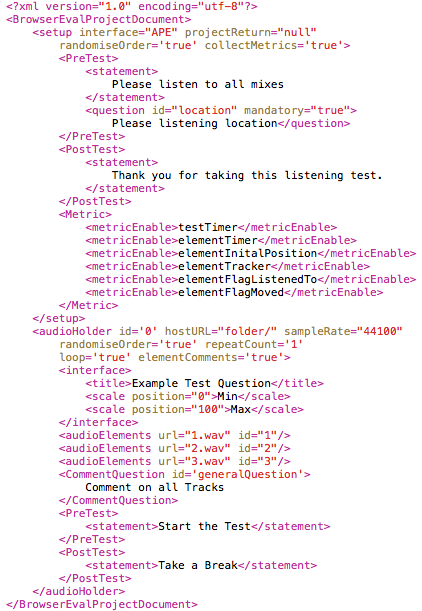
\includegraphics[width=0.5\textwidth]{XMLInput.png}
\caption{An Example Input XML File}
\label{fig:xmlIn}
\end{center}
\end{figure}

The set up document has several defined nodes and structure which are documented with the source code. For example there is a section for general set up options where the pre-test and post-test questions and statements are set up and from the example in Figure~\ref{fig:xmlIn}, it can be seen that a question box should be generated, with the id 'location' and it is mandatory to answer. The question is in the PreTest node meaning it will appear before any testing will begin. When the result for the  entire test is shown, then this will appear in the PreTest node of the response with the id 'location' allowing it to be found easily. This outlines the importance of having clear and meaningful ID values. Pre- and post-test dialog boxes allow for comments or questions to be presented before or after the test, to convey listening test instructions, gather information about the subject, listening environment, and overall experience of the test.
 

We try to cater to a diverse audience with this toolbox, while ensuring the toolbox is simple, elegant and straightforward. To that end, we include the following options that can be easily switched on and off, by setting the value in the input XML file. 

\begin{itemize} %Should have used a description list for this.
\item \textbf{Snap to corresponding position}: When this is enabled, and a fragment is playing, the playhead skips to the same position in the next fragment that is clicked. If it is not enabled, every fragment is played from the start. 
\item \textbf{Loop fragments}: Repeat current fragment when end is reached, until the `Stop audio' or `Submit' button is clicked. 
\item \textbf{Comments}: Displays a separate comment box for each fragment in the page.
\item \textbf{General comment}: One comment box, additional to the individual comment boxes, to comment on the test or a feature that some or all of the fragments share. 
\item \textbf{Resampling}: When this is enabled, tracks are resampled to match the subject's system's sample rate (a default feature of the Web Audio API). When it is not, an error is shown when the system does not match the requested sample rate. 
\item \textbf{Randomise page order}: Randomises the order in which different `pages' are presented. % are we calling this 'pages'?
\item \textbf{Randomise fragment order}: Randomises the order and numbering of the markers and comment boxes corresponding with the fragments. This permutation is stored as well, to be able to interpret references to the numbers in the comments (such as `this is much [brighter] then 4'). 
\item \textbf{Require playback}: Require that each fragment has been played at least once, if not in full. 
\item \textbf{Require full playback}: If `Require playback' is active, require that each fragment has been played in full. 
\item \textbf{Require moving}: Require that each marker is moved (dragged) at least once. 
\item \textbf{Require comments}: This option allows requiring the subject to require a comment for each track. 
\item \textbf{Repeat test}: Number of times test should be repeated (none by default), to allow familiarisation with the content and experiment, and to investigate consistency of user and variability due to familiarity. In the set up, each 'page' can be given a repeat count. These are all gathered before shuffling the order so repeated tests are not back-to-back if possible.
\item \textbf{Returning to previous pages}: Indicates whether it is possible to go back to a previous `page' in the test. 
\item \textbf{Lowest rating below [value]}: To enforce a certain use of the rating scale, it can be required to rate at least one sample below a specified value. 
\item \textbf{Highest rating above [value]}: To enforce a certain use of the rating scale, it can be required to rate at least one sample above a specified value. 
\item \textbf{Reference}: Allows for a separate sample (outside of the axis) to be the `reference', which the subject can play back during the test to help with the task at hand \cite{mushra}. 
\item \textbf{Hidden reference}: Whether or not an explicit `reference' is provided, the `hidden reference' should be rated above a certain value \cite{mushra} - this can be enforced. 
\item \textbf{Hidden anchor}: The `hidden anchor' should be rated lower than a certain value \cite{mushra} - this can be enforced. 
\end{itemize}

When one of these options is not included in the set up file, they assume a default value. As a result, the input file can be kept very compact if default values suffice for the test.  

% loop, snap to corresponding position, comments, 'general' comment, require same sampling rate, different types of randomisation

\subsection{Results}

The results file is dynamically generated by the interface upon clicking the `Submit' button. This also executes checks, depending on the set up file, to ensure that all tracks have been played back, rated and commented on. The XML output returned contains a node per audioObject and contains both the corresponding marker's position and any comments written in the associated comment box. The rating returned is normalised to be a value between 0 and 1, normalising the pixel representation of different browser windows. An example output file is presented in Figure~\ref{fig:xmlOut}

\begin{figure}[ht]
\begin{center}
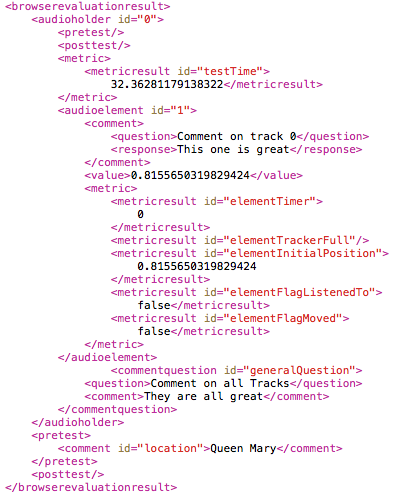
\includegraphics[width=0.5\textwidth]{XMLOutput.png}
\caption{An Example Output XML File}
\label{fig:xmlOut}
\end{center}
\end{figure}

The results also contain information collected by any defined pre/post questions. These are referenced against the set up XML by using the same ID so readable responses can be obtained. Taking from the earlier example of setting up a pre-test question, an example response can be seen in Figure \label{fig:xmlOut}.

Each page of testing is returned with the results of the entire page included in the structure. One `audioElement' node is created per audio fragment per page, along with its ID. This includes several child nodes including the value holding the rating between 0 and 1, the comment, and any other collected metrics. The latter include how long the element was listened for, the initial position, boolean flags if the element was listened to, if the element was moved and if the element comment box had any comment. Furthermore, each user action (manipulation of any interface element, such as playback or moving a marker) is logged along with a the corresponding time code and stored or sent along with the results.
Furthermore, we also store session data such as the browser the tool was used in. 

We provide the option to store the results locally, and/or to have them sent to a server. 

%Here is an example of the set up XML and the results XML: % perhaps best to refer to each XML after each section (set up <> results)
% Should we include an Example of the input and output XML structure?? --> Sure. 

%An example of the returned \textit{audioElement} node in the results XML file is as follows.
%
%\texttt{<audioelement id="8"> \\
%<comment> \\
%<question>Comment on track 0</question> \\
%<response> The drums were punchy </response> \\
%</comment> \\
%<value> 0.25169491525423726 </value> \\
%<metric> \\
%<metricresult id="elementTimer"> \\ 2.3278004535147385< /metricresult> \\
%<metricresult id="elementTrackerFull"> \\
%<timepos id="0"> \\
%<time>1.7937414965986385</time> \\
%<position>0.41694915254237286</position> \\
%</timepos> \\
%<timepos id="1"> \\
%<time>2.6993197278911563</time> \\
%<position>0.45847457627118643</position> \\
%</timepos> \\</metricresult> \\
%<metricresult id="elementInitialPosition"> 0.47796610169491527 </metricresult> \\
%<metricresult id="elementFlagListenedTo"> true< /metricresult> \\
%<metricresult id="elementFlagMoved"> true </metricresult> \\
%</metric> \\
%</audioelement>}

As can be seen from Figure~\ref{fig:xmlOut}, the parent tag \texttt{audioelement} holds the id of the element passed in from the set up document. The first child element is \texttt{comment} and holds both the question shown and the response from the comment box inside. 
The child element \texttt{value} holds the normalised ranking value. Next comes the metric node structure, there is one \texttt{metricresult} node per metric event collected. The id of the node identifies the type of data it contains. For example, the first holds the id \textit{elementTimer} and the data contained represents how long, in seconds, the audio element was listened to. The next holds the id \textit{elementTrackerFull} and contains a pair of elements per entry. This represents the entire movement of the elements' slider giving the time the event took place in seconds from when the current test page started, and the new position. In our example there are three \texttt{timepos} children with their id representing their order. There is one of these \texttt{audioelement} tags per audio element outlined on each test page. 


\section{Conclusions and future work}\label{sec:conclusions}

In this paper we have presented an approach to creating a browser-based listening test environment that can be used for a variety of types of perceptual evaluation of audio. 
Specifically, we discussed the use of the toolbox in the context of assessment of preference for different production practices, with identical source material. 
The purpose of this paper is to outline the design of this tool, to describe our implementation using basic HTML5 functionality, and to discuss design challenges and limitations of our approach. % or something

% future work
Further work may include the development of other common test designs, such as MUSHRA \cite{mushra}, 2D valence and arousal rating, and others. We will add functionality to assist with setting up large-scale tests with remote subjects, so this becomes straightforward and intuitive. 
In addition, we will keep on improving and expanding the tool, and highly welcome feedback and contributions from the community. 

The source code of this tool can be found on \url{code.soundsoftware.ac.uk/projects/webaudioevaluationtool}. 


%%%%%%%%%%%%%%%%%%%%%%%%%%%%%%%%%%%%%%%%%%%%%%%%%%%%%%%%%%%%%%%%%%%%%%%%%%%%%
%bibliography here
\bibliography{smc2015template}

\end{document}
